\setlength{\parindent}{0in}	% disable indentation

\chapter{Additional tools installation instructions}
\label{cha:additionalToolsInstallationInstructions}

\section{Protégé installation}
\label{sec:protegeInstallation}

\subsection{Editor installation}
\label{sub:editorInstallation}

The installation instructions can be found on Protégé home page \cite{ProtegeHome}. First, download the latest version of Protégé tool from the Protégé home page. Choose installation variant based on your system type.

\bigskip

{\scshape Windows}
\smallskip

After downloading double-click \texttt{install\_protege\_4.0.2.exe}.
\smallskip

\begin{framed}
If you do not have a Java virtual machine installed, be sure to download the package above which includes one. 
\end{framed}

\bigskip

{\scshape Linux}
\smallskip

After downloading open a shell and go to the directory of downloaded installer. At the prompt type:  
\begin{verbatim}
sh ./install_protege_4.0.2.bin 
\end{verbatim}

\begin{framed}
If you do not have a Java virtual machine installed, be sure to download the package above which includes one. Otherwise you may need to download one from Sun's Java website \cite{SunHome} or contact your OS manufacturer. 
\end{framed}

\newpage
{\scshape All other platforms}

\begin{enumerate}
    \setlength{\itemsep}{0cm}
    \setlength{\parskip}{0cm}

    \item Instructions for Unix or Unix-like operating systems
    \begin{itemize}
        \setlength{\itemsep}{0cm}
        \setlength{\parskip}{0cm}

        \item For Java 2, after downloading, type
\begin{verbatim}
java -jar install_protege_4.0.2.jar
\end{verbatim}
        \item For Java 1.1, after downloading, type
\begin{verbatim}
jre -cp install_protege_4.0.2.jar install
\end{verbatim}
        \item If that does not work, try
\begin{verbatim}
java -classpath [path to] classes.zip:install_protege_4.0.2.jar install
\end{verbatim}
        \item If that does not work either, on sh-like shells, try
\begin{verbatim}
cd [to directory where install_protege_4.0.2.jar is located]
CLASSPATH=install_protege_4.0.2.jar
export CLASSPATH
java install
\end{verbatim}
        \item Or for csh-like shells, try
\begin{verbatim}
cd [to directory where install_protege_4.0.2.jar is located]
setenv CLASSPATH install_protege_4.0.2.jar
java install
\end{verbatim}
    \end{itemize}
    \item Instructions for other platforms
    \begin{itemize}
        \setlength{\itemsep}{0cm}
        \setlength{\parskip}{0cm}

        \item Be sure you have Java installed. You can download Java from Sun's website \cite{SunHome}.
        \item In a console window, change to the directory where you downloaded \texttt{install\_protege\_4.0.2.jar} to before running the installer.
    \end{itemize}
\end{enumerate}

Your operating system may invoke Java in a different way. To start the installer, add \texttt{install\_protege\_4.0.2.jar} to your \texttt{CLASSPATH}, then start the main class of the installer named \texttt{install}.

\newpage
\subsection{Plugins installation}
\label{sub:pluginsInstallation}

After installation of Protégé there can be custom need of installation additional plugins. For plugins installation go to \textit{File->Preferences->Plugins} tab and click \textit{Check for downloads now} button (Figure \ref{fig:plugins}). 

\medskip

\begin{figure}[htp]
\centering
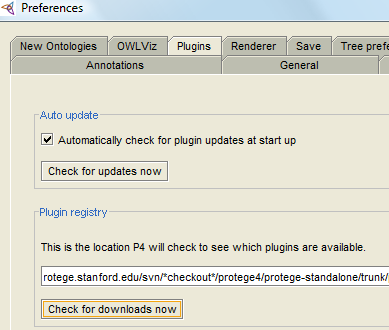
\includegraphics[scale=0.7]{images/appendixA/PreferencesPlugins}
\caption{Plugins tab}
\label{fig:plugins}
\end{figure}

For all additional instructions check the wiki page for Protégé \cite{ProtegeWiki}. That is very competitive and reliable source of all information that may be needed. It includes documentation, tutorials, sample ontologies, plugin libraries, etc.

\section{Maven installation}
\label{sec:mavenInstallation}

Maven will be very helpful while working with sources of the project, because it can automatically download all dependencies tree from the network.

\bigskip

Maven is a Java tool, so you must have Java installed in order to proceed. Java Development Kit (JDK) is required (Java Runtime Environment (JRE) is not sufficient). Installation instructions provided below can be found on Maven home page \cite{MavenHome}.

\newpage

{\scshape Windows}

\begin{enumerate}
    \setlength{\itemsep}{0cm}
    \setlength{\parskip}{0cm}

    \item Download the latest Maven archive from Maven home page and unzip the distribution archive, i.e. \texttt{apache-maven-2.2.1-bin.zip} to the directory you wish to install Maven 2.2.1. These instructions assume you chose \path{C:\Program Files\Apache Software Foundation\}.
    \item Add the \texttt{M2\_HOME} environment variable by opening up the system properties (\texttt{WinKey+Pause}), selecting the \textit{Advanced} tab, and the \textit{Environment Variables} button, then adding the \texttt{M2\_HOME} variable in the user variables with the value \path{C:\Program Files\Apache Software Foundation\apache-maven-2.2.1}.
    \item In the same dialog, add the \texttt{M2} environment variable in the user variables with the value \path{%M2_HOME%\bin}.
    \item In the same dialog, update/create the \texttt{PATH} environment variable in the user variables and prepend the value \texttt{\%M2\%} to it (in order to make Maven available in the command line).
    \item In the same dialog, make sure that \texttt{JAVA\_HOME} exists in your user variables or in the system variables and it is set to the location of your JDK, e.g. \path{C:\Program Files\Java\jdk1.5.0_02} and that \path{%JAVA_HOME%\bin} is in your \texttt{PATH} environment variable.
\end{enumerate}

{\scshape Unix-based operating systems}

\begin{enumerate}
    \setlength{\itemsep}{0cm}
    \setlength{\parskip}{0cm}

    \item Download the latest Maven archive from Maven home page and unzip the distribution archive, i.e. \texttt{apache-maven-2.2.1-bin.zip} to the directory you wish to install Maven 2.2.1. These instructions assume you chose \path{/usr/local/apache-maven/}. The subdirectory \texttt{apache-maven-2.2.1} will be created from the archive.
    \item In a command terminal, add the \texttt{M2\_HOME} environment variable, e.g.
\begin{verbatim}
export M2_HOME=/usr/local/apache-maven/apache-maven-2.2.1
\end{verbatim}
    \item Add the \texttt{M2} environment variable, e.g. 
\begin{verbatim}
export M2=$M2_HOME/bin
\end{verbatim}
    \item Add \texttt{M2} environment variable to your path, e.g. 
\begin{verbatim}
export PATH=$M2:$PATH
\end{verbatim}
    \item Make sure that \texttt{JAVA\_HOME} is set to the location of your JDK, e.g. 
\begin{verbatim}
export JAVA_HOME=/usr/java/jdk1.5.0_02
\end{verbatim}
and that \path{$JAVA_HOME/bin} is in your \texttt{PATH} environment variable.   
\end{enumerate}
